\documentclass[a4paper]{article}

%% The graphicx package provides the includegraphics command.
\usepackage{graphicx}
\usepackage{caption}
\usepackage{subcaption}
\usepackage{multirow}
\usepackage{biblatex}
\addbibresource{ref.bib}
%% The amsthm package provides extended theorem environments
\usepackage{amssymb}
\usepackage{amsthm}
\usepackage{amsmath}
\usepackage{bm}
\usepackage{fancyvrb}
\usepackage{dsfont}
\usepackage{float}
\usepackage[utf8]{inputenc}
\usepackage{bbm}
\usepackage{amsmath}
\usepackage{bbold}
\usepackage{algorithm}
\usepackage[noend]{algpseudocode}
\usepackage{algorithmicx}
\usepackage{algpseudocode}
\usepackage{stackengine}
\usepackage{amsmath}               
  {
      \theoremstyle{plain}
      \newtheorem{assumption}{M}
      \newtheorem{assumption_saem}{SAEM}
  }
\usepackage{amssymb,amsthm,mathrsfs,amsfonts,dsfont}
\DeclareMathOperator*{\E}{\mathbb{E}}
\DeclareMathOperator*{\s}{\barbelow{s}}
\theoremstyle{plain}
\newtheorem{thm}{Theorem}

\theoremstyle{definition}
\newtheorem{defn}[thm]{Definition} % definition numbers are dependent on theorem numbers
\newtheorem{exmp}[thm]{Example} % same for example numbers
\newcommand{\Pt}{\~P}
\newcommand\barbelow[1]{\stackunder[1.2pt]{$#1$}{\rule{.8ex}{.075ex}}}
%% remove journal footer
\makeatletter
\def\ps@pprintTitle{%
 \let\@oddhead\@empty
 \let\@evenhead\@empty
 \def\@oddfoot{}%
 \let\@evenfoot\@oddfoot}
\makeatother


%% change 'Abstract' to 'Outline'
\renewenvironment{abstract}{\global\setbox\absbox=\vbox\bgroup
  \hsize=\textwidth\def\baselinestretch{1}%
  \noindent\unskip\textbf{Outline}
 \par\medskip\noindent\unskip\ignorespaces}
 {\egroup}



\begin{document}
\pagenumbering{gobble}

\Large
 \begin{center}
Incremental Stochastic EM In Practice

\hspace{10pt}

% Author names and affiliations
\large
Belhal Karimi

\hspace{10pt}

\end{center}

\hspace{10pt}

\normalsize

%% main text


 \noindent The Monte Carlo EM (MCEM) and the Stochastic Approximation EM (SAEM) are powerful inference algorithm in the context of missing data models. We introduce variants of those algorithms that justifies incremental versions where only one, or a batch of individuals, are considered at each iteration. In both cases we'll prove almost-sure convergence and give experimental results on simple cases and on more complicated Pharmacokinetics models showing the effectiveness of our technique.


\section{Introduction}
We consider a complete model (y,z) where the realizations of y are observed and z is the missing data. When the complete model $p(y,z,\theta)$ is parametric, the goal is to compute the maximum likelihood (ML) estimate of the parameter of this joint distribution.
\begin{equation}
\theta^{ML} = \arg\max p(Y,\theta)
\end{equation}
When the direct derivation of this expression is hard, several methods use the complete model to iteratively find the quantity of interest.
The EM algorithm has been the object of considerable interest since its presentation by Dempster, Laird and Rubin in 1977. It has been relatively effective in context of maximum likelihood estimation of parameters of incomplete model (unobserved or more). This algorithm is monotonic in likelihood making it a stable tool to work with.

Many improvements have been provided since the birth of this algorithm. In particular, \citep{neal} proposed an incremental version where a single data is handled at each iteration. It showed faster convergence accompanied by a lost of monotonic convergence in likelihood.\\
In terms of efficiency of computation, \citep{fort, cappe} introduced an online version where the whole dataset is not analyzed at each iteration but a growing batch of it only.

Yet, when the quantity computed at the E-step involves infeasible computations, new methods have been developed in order to by-pass the issue. The stochastic EM algorithm \citep{diebolt} has been proposed in the context of mixture problem and involves splitting the E-step in a first simulation of the latent variables step and then a direct evaluation of the complete log model. A Robbins Monroe type approximation can be used to evaluate that latter quantity after the simulation step, that is the SAEM algorithm \citep{lavielle2,moulines}.
Based on that last derivation of the EM algorithm, we are presenting a view that justifies an incremental variant of the SAEM algorithm and how these versions can be implemented in practice.\\
Many questions arise when a choice of subset of the overall dataset is at stake at each iteration. Indeed, one can wonder how many individuals to consider at each iteration. Even though historical version of the Incremental EM algorithm by NEal and Hinton involves one individual per iteration, we'll show that the size of the batch is influencing the outcome for both determinstic and stochastic versions. Moreover, the other aspect we will introduce in this document relates to the indices choice strategy adopted for each algorithm. This strategy can be shown to be efficient when changing through the iterations.



%------------------------------------------------


\section{Model and notations}
We study a classical missing data problem where:
\begin{itemize}
\item y is a random variable called the observed data that takes its value in $(y_i, 1\leq i \leq N)$
\item z represents the missing data and takes its value in$(z_i, 1\leq i \leq N)$
\item $\log p(y,\theta)$ is the incomplete data log-likelihood
\item $\log p(y,z,\theta)$ is the complete data log-likelihood (y,z) and obtained by augmenting the observed data with the missing data
\end{itemize}


In this article, we are restricting ourselves to models that belong to the curved exponential family:
\begin{assumption}
$\Theta \subseteq \mathbb{R}^l$ the parameter space, $ \mathcal{Y} \subseteq \mathbb{R}^d$ and $\mathcal{Z} \subseteq \mathbb{R}^d$ and $\mu$ is a $\sigma$-finite positive Borel measure on $\mathcal{Y} \times \mathcal{Z}$.\\
Denote by $\langle . { , }. \rangle$ the scalar product.
\begin{equation}
\log p(y_i,z_i,\theta) = -\psi(\theta) + \langle S(y_i,z_i), \phi(\theta)\rangle
\end{equation}
\end{assumption}
Where $\psi$, $\phi$ are continuous function of $\theta$ and S is a sufficient statistic of the complete model which takes its values in an open subset $\mathcal{S}$ of $\mathbb{R}$. In the sequel, the incomplete and the complete likelihood, with respect to the reference measure $\mu$ will be noted as $l(\theta)$ and $L(s,\theta)$\\
We assume the continuity of the incomplete log-likelihood. 

\begin{assumption}
\begin{itemize}
\item $\psi$, $\phi$ are continuous on $\Theta$and S is continuous on $\mathcal{Y} \times \mathcal{Z}$
\item $\forall \theta \in \Theta, \bar{S}(\theta):= p(z|y,\theta)\mu(dz) = \frac{p(y,z,\theta)}{p(y,\theta)}\mu(dz)$ is finite and continuous on $\Theta$
\item There exists a continuous function $\hat{\theta}: \mathcal{S} \mapsto \Theta$ such that for all $s \in \mathcal{S}$, $L(s,\hat{\theta}(s)) = \sup L(s,\theta)$
\item $p(y,\theta)$ is a continuous function of $\theta$ and for any $M > 0$ the level set $\{\theta \in \Theta, p(y,\theta) > M\}$ is compact
\end{itemize}
\end{assumption}


Let denote the stationary points of the EM algorithm as $\mathcal{L}$. Every point in $\mathcal{L}$ is thus a stationary point of the function $\hat{\theta}(S)$ as defined above.
\begin{assumption}
$p(y,\mathcal{L})$ is compact
\end{assumption}
%------------------------------------------------

\section{Maximum likelihood estimation}
Our problem joins a familiar class of problem in computational statistics that consists in maximizing the following quantity:
\begin{equation}
\log p(y,\theta) = \int_{}{\log p(y,z,\theta)\mu(dz)}
\end{equation}
When this quantity can not be computed in closed form, many algorithms use iterative procedure to find the maximum likelihood parameter estimate. Among those techniques, the EM algorithm \citep{dempster}. This two steps algorithm consists in maximizing an auxiliary quantity that is the expectation of the complete log-likelihood with respect to the conditional distribution over the missing variable conditioned on the current parameter estimate (also called the posterior distribution).\\
Several alternatives have been developed throughout the past decades. Most of them alleviate the computation of the expectation using approximates. The MCEM algorithm \citep{diebolt} approximate this quantity by a Monte Carlo integration, the SAEM algorithm \citep{lavielle} uses a stochastic approximation of this quantity.\\
In this paper we'll deal with the incremental versions of those three algorithms (EM, MCEM and SAEM) noted IEM, IMCEM and ISAEM.
\\
First let's explain how the incremental version of the EM algorithm can be shown to converge.\\
Following \citep{byrne} work, it is important to introduce this algorithm as an iteration of two minimizations over two different spaces.

\section{Implementing the Incremental SAEM}
In this section we will deal with all the specifities of implementing incremental stochastic versions of the EM algorithm. On synthetic data, but also on real pharmakokinetics data and models, our practical implementations of those algorithm are going to highlight several aspect that could make the behaviour of convergence different.\\
Let's start with a simple example.

\subsection{Simple case}

Let's consider the case when all the variables of interest are Gaussian.
\begin{equation}
y_i = z_i + \epsilon_i
\end{equation}
Where $z_i \sim \mathcal{N}(\theta,\omega^2)$ and $\epsilon_i \sim \mathcal{N}(0,\sigma^2)$.
Since the $z_i$ and $\epsilon_i$ are i.i.d we have that $y_i \sim \mathcal{N}(\theta,\sigma^2 + \omega^2)$ and $y_i|z_i \sim \mathcal{N}(z_i,\sigma^2)$.\\
The goal is to find an estimate of the mean $\theta$ that maximizes the likelihood $p(y,\theta)$ considering that $\sigma^2$ and $\epsilon^2$ are known. The maximum likelihood is easy to compute in this case since $y_i \sim \mathcal{N}(\theta,\sigma^2 + \omega^2)$:
\begin{equation}
\theta_{ML} = \frac{1}{N}\sum_{i=1}^{N}{y_i}
\end{equation}\\

We can rewrite the complete log likelihood $\log p(y,z,\theta)$ as part of the exponential family:
\begin{equation}
\begin{split}
\log p(y,z,\theta) & = \sum_{i=1}^{N}{(\log p(y_i|z_i,\theta) + \log p(z_i,\theta))}\\
& = \sum_{i=1}^{N}{-\frac{1}{2}\log(2\pi\sigma^2) -\frac{(y_i - z_i)^2}{2\sigma^2} -\frac{1}{2}\log(2\pi\omega^2) -\frac{(z_i - \theta)^2}{2\omega^2}}
\end{split}
\end{equation}
The resulting statistics are: $S_1(y,z) = \sum_{i=1}^{N}{z_i} $, $S_2(y,z) = \sum_{i=1}^{N}{z_iy_i} $,$S_3(y,z) = \sum_{i=1}^{N}{z_i^2} $
Let's define the quantity of interest $p(z_i|y_i,\theta)$ using Bayes rule.
We find that $z_i|y_i \sim \mathcal{N}(\alpha\theta+(1-\alpha)\bar{y}, \Gamma^2)$ with $\alpha = \frac{\sigma^2}{\sigma^2+\omega^2}$ and $\Gamma^2 = \frac{\sigma^2\omega^2}{\sigma^2+\omega^2}$


\subsubsection{EM}
Let's use the alternating minimization framework. At iteration $k+1$ we do:\\
\textbf{Forward mapping:} Find the distribution that minimizes the criteria as defined above.\\
It is well known that $p(z|y,\theta_k)$ is the solution of our minimization problem.

\noindent \textbf{Backward mapping:}
\begin{equation}
\begin{split}
& \theta_{k+1} = \arg \max \limits_{\theta \in \Theta} \E_{p(z|y,\theta_k)}(p(y,z,\theta))\\
& = \hat{\theta}(S) = \frac{\sum_{i=1}^{N}{\E{(S(y_i,z_i)|y_i,\theta_{k})}}}{N}\\
& = \alpha \theta_{k} + (1-\alpha)\bar{y}\\
& \theta_{k+1} - \hat{\theta} = \alpha (\theta_{k} - \hat{\theta})\\
& \theta_{k+1} - \hat{\theta} = \alpha^{k+1} (\theta_{0} - \hat{\theta})
\end{split}
\end{equation}

Since $\alpha < 1$, the convergence is proven

\subsubsection{IEM}
Here the vector of sufficient statistic is different because at each iteration only one individual is picked.\\
It is necessary that one pass over the data has already been done. We are then dealing with any iterations $N+j$ where we pick individual $j$ only.

\begin{equation}
S(y,z) = 
\left(
\begin{array}{c}
S(y_1,z_1) =z_1^{(N+j)}= z_1^{(N+1)}\\
..\\
S(y_j,z_j) =z_j^{(N+j)}= z_j^{(N+j)}\\
..\\
S(y_N,z_N) =z_N^{(N+j)}= z_N^{(N)}\\
\end{array}
\right)
\end{equation}
\noindent The Forward mapping gives us the expression of the expectation of each component of the sufficient statistic:
\begin{equation}
\begin{matrix} 
\E_{Q_1^{(N+j)}}(z_1^{(N+j)})= \E_{Q_1^{(N+1)}}(z_1^{(N+1)})=\E_{p(z_1|y_1,\theta_N)}(z_1^{(N+1)}) = \alpha \theta_{N} + (1-\alpha)y_1\\
..\\
\E_{Q_j^{(N+j)}}(z_j^{(N+j)})=\E_{p(z_j|y_j,\theta_{N+j-1})}(z_j^{(N+j)})= \alpha \theta_{N+j-1} + (1-\alpha)y_j\\
..\\
\E_{Q_N^{(N+j)}}(z_N^{(N+j)})= \E_{Q_N^{(N)}}(z_N^{(N)})=\E_{p(z_N|y_N,\theta_{N-1})}(z_N^{(N)}) = \alpha \theta_{N-1} + (1-\alpha)y_N
\end{matrix}
\end{equation}

\noindent We can now apply our maximization step:
\begin{equation}
\begin{split}
& \theta_{(N+j)} = \hat{\Theta}(S) = \frac{\sum_{i=1}^{N}{\E{(S(y_i,z_i)|y_i,\theta_{(N+j-i)})}}}{N}\\
& \theta_{(N+j)} = \frac{\alpha}{N} \sum_{i=1}^{N}{\theta_{N+j-i}} + (1-\alpha)\bar{y}\\
\end{split}
\end{equation}

We can rewrite this expression as follows:

\begin{equation}
\begin{split}
\theta_{(k,j)} &  = \hat{\Theta}(S) = \frac{\sum_{i=1}^{N}{\E{(S(y_i,z_i)|y_i,\theta_{(k,j-1)})}}}{N}\\
& = \frac{1}{N}(\alpha \theta_{(k,j-1)} + (1-\alpha)y_j + \sum_{i \neq j}^{}{\E{(S(y_i,z_i)|y_i,\theta_{(k,j-1)})}})\\
& = \frac{1}{N}(\alpha \theta_{(k,j-1)} + (1-\alpha)y_j) + \theta_{(k,j-1)} - \frac{1}{N}(\alpha \theta_{(k-1,j)} + (1-\alpha)y_j)\\
& =  \theta_{(k,j-1)} + \frac{\alpha}{N}(\theta_{(k,j-1)} - \theta_{(k-1,j)}) 
\end{split}
\end{equation}

Because of the monotony of the parameter estimate evolution curve, we can affirm that the difference $\theta_{(k,j-1)} - \theta_{(k-1,j)}$ is maximal at its value $\theta_{(k,i)} - \theta_{(k-1,i)}$ when i is picked sequentially and not uniformly for instance.\\

See graphs\\
\begin{figure}[H]
\begin{center}
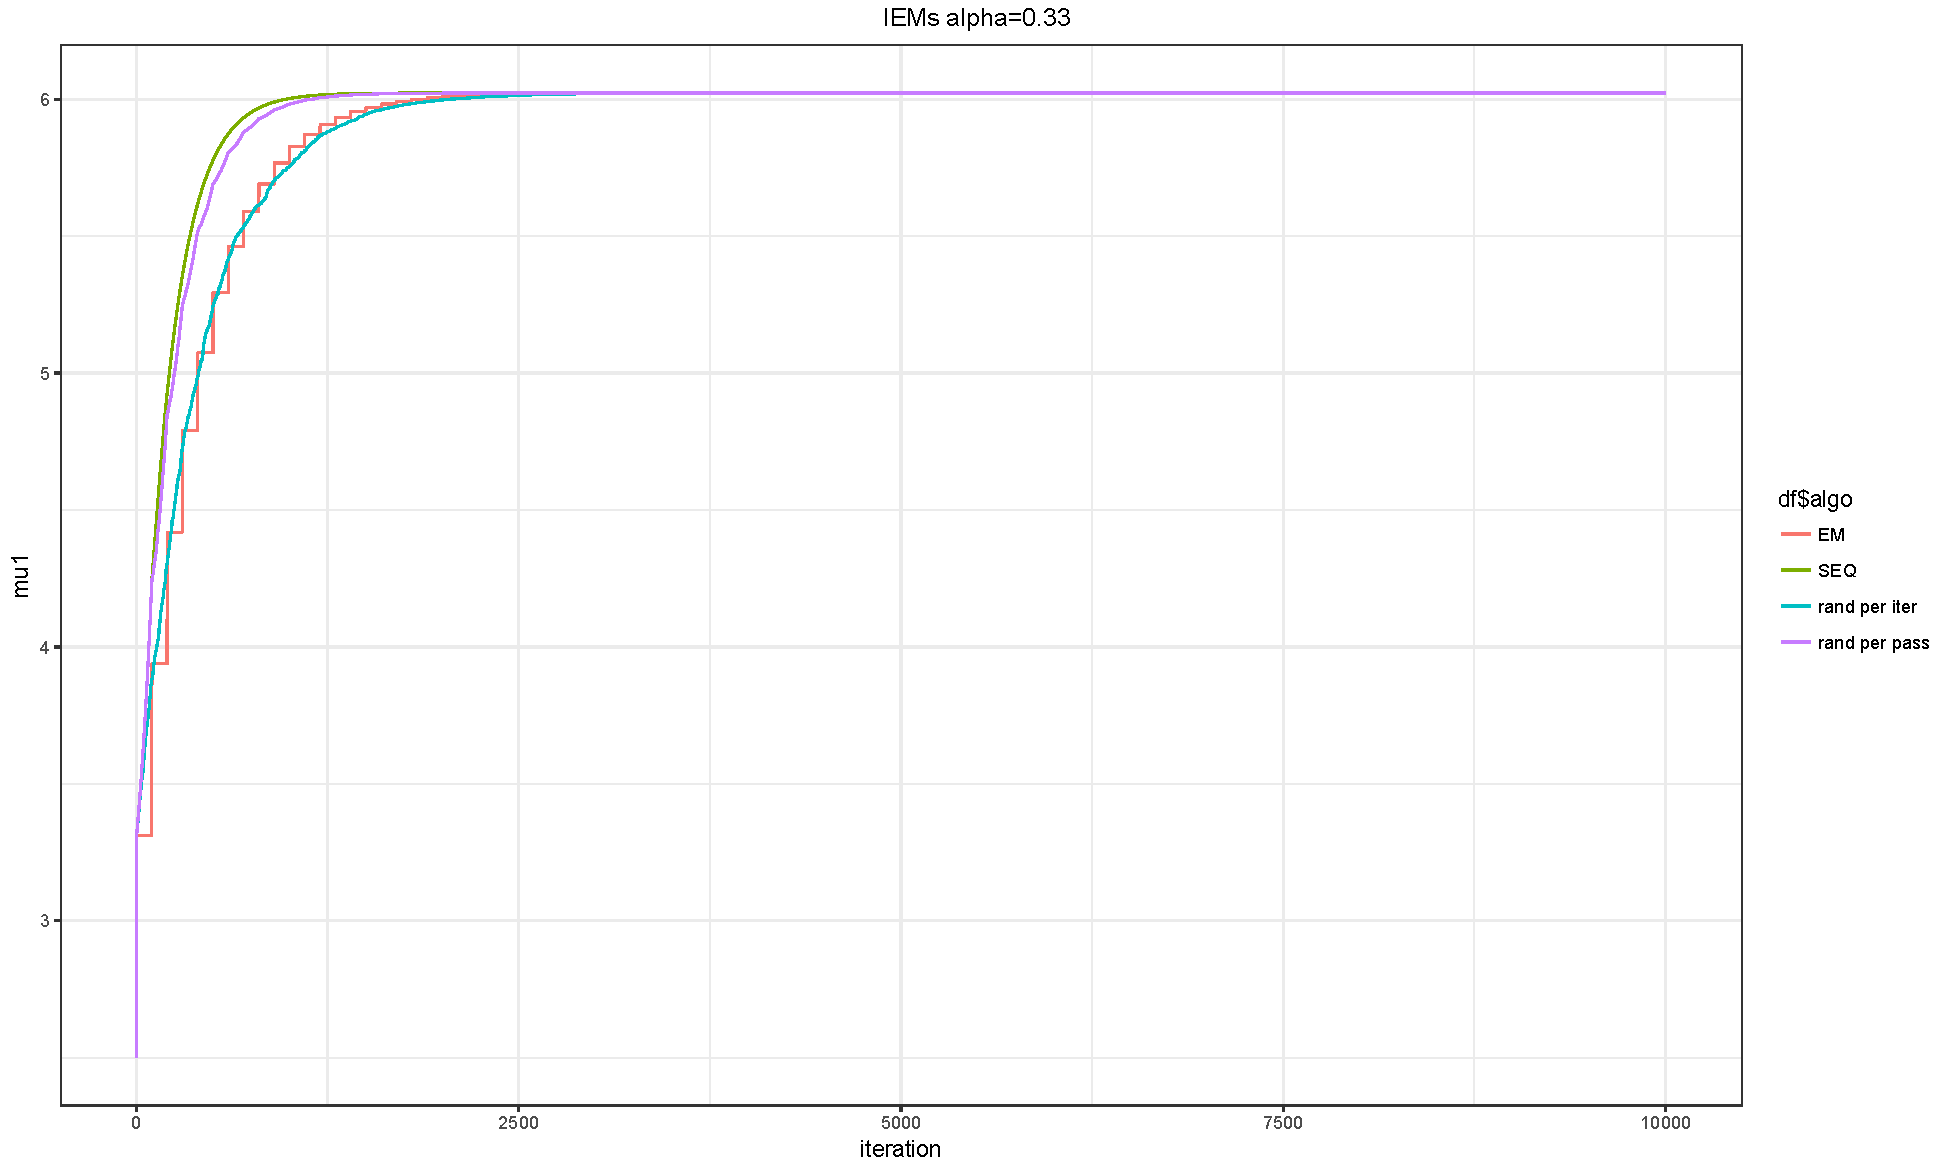
\includegraphics[scale=0.3]{iem.pdf}
\end{center}
\end{figure}





If we rewrite the recurrent relation between paramter estimates when we pick half of the individuals at each iteration (and not just one).
\begin{equation}
\begin{split}
\theta_{(k,j)} &  = \hat{\Theta}(S) = \frac{\sum_{i=1}^{N}{\E{(S(y_i,z_i)|y_i,\theta_{(k,j-1)})}}}{N}\\
& =  \theta_{(k,j-1)} + \frac{\alpha}{2}(\theta_{(k,j-1)} - \theta_{(k-1,j)}) 
\end{split}
\end{equation}

It's important to keep in mind that in the first scenario, a pass from $k-1$ to $k$ was N iterations whereas here it's only $2$.\\
\textbf{Gauss-Southwell rule}\\
This rule consists in taking at each iteration the individual indice that present the highest gradient in the case of a stochastic gradient algorithm for instance.\\
We decided to follow this rule to show optimality of the IEM whith sequential picking of only one individual at each iteration. 
\subsubsection{3 components gaussian mixture}
To highlight this last point, we'll need to work on the gaussian mixture example.\\
Our implementation of the Gauss Southwell rule is as follow:


\begin{algorithm}
    \caption{PIEM Algorithm}
    \label{alg:pseudoPIEM}
    \begin{algorithmic}[1]
    \State Initial value $\theta_0$
    \State $\theta \gets \theta_0$
    \State $p_{j} \gets (p_{ij}(\theta_0),1\leqslant i \leqslant N)$
    \For{$k \gets 1 \textrm{ to } K$}
        \For{$i \gets 1 \textrm{ to } n$}
        \State $p_{ij}(\theta) \gets \frac{\pi_jf(y_i;\theta_j)}{\sum_{l=1}^{J}\pi_lf(y_i;\theta_l)}$
        \EndFor  
        \State $i' \gets \max\limits_{i}\{(p^{(k)}_{ij}-p^{(k-1)}_{ij})^2\}$
        \State $p_{i'j}(\theta) \gets \frac{\pi_jf(y_i;\theta_j)}{\sum_{l=1}^{J}\pi_lf(y_i;\theta_l)}$
        \State $s_k \gets ((\sum_{i=1}^{n}{p_{i'j}}),(\sum_{i=1}^{n}{p_{ij}y_i}),(\sum_{i=1}^{n}{p_{ij}y_i^2}))$
        \State $\theta_k \gets \Theta(s_k)$
    \EndFor  
    \State \Return $\theta_K$
    \end{algorithmic}
\end{algorithm}

As described, the optimal version of the IEM consists in always choosing the individual that made the prior distribution progress the most (or the highest poseterior distribution, in norm). This relates to the GS-rule since:
\begin{equation}
p_{ij} = \frac{\pi_jf(y_i;\theta_j)}{\sum_{l=1}^{J}\pi_lf(y_i;\theta_l)} = \pi_j \frac{\partial log p}{\partial \pi_j}
\end{equation}

\begin{figure}[H]
\begin{center}
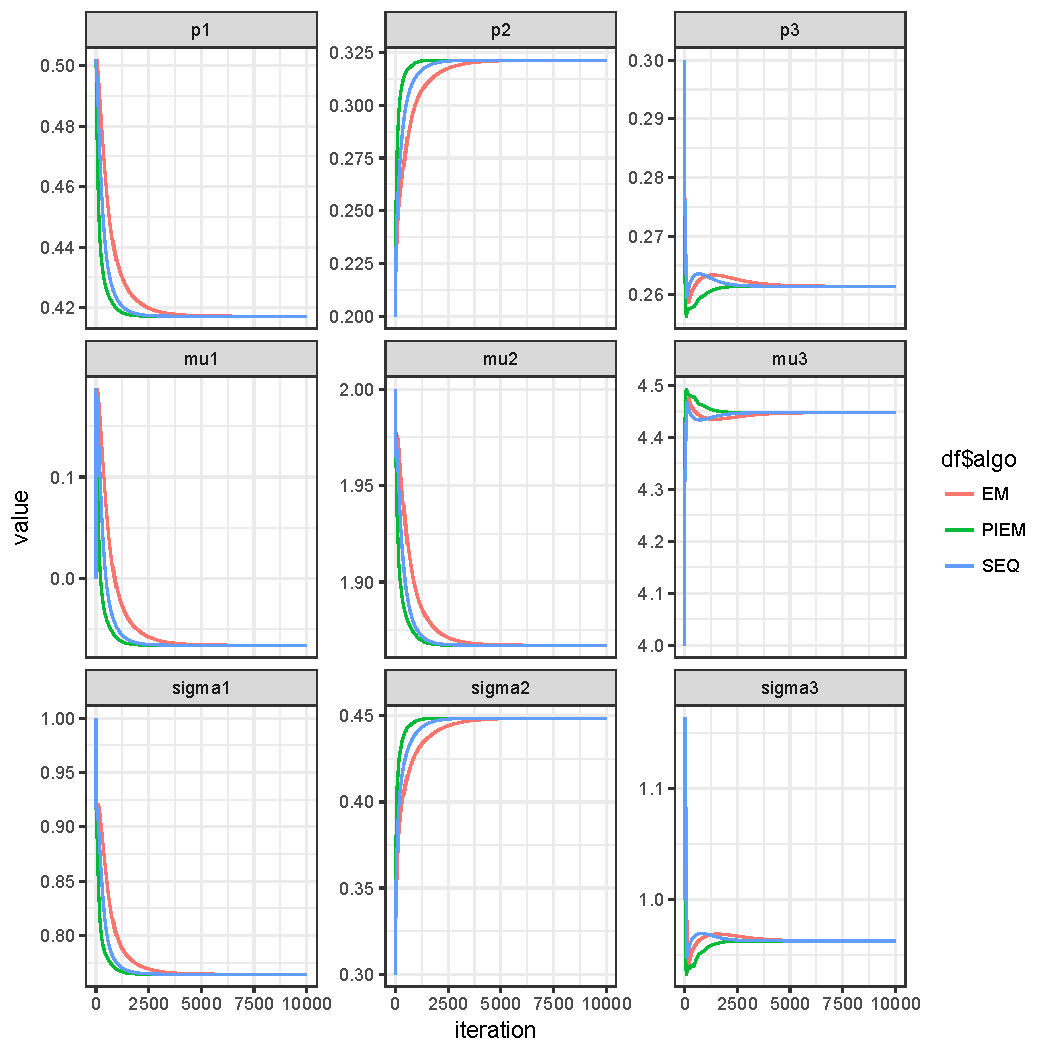
\includegraphics[scale=0.5]{piem_2gmm.pdf}
\end{center}
\end{figure}


The same algorithm on the prior simple case shows no improvment since the sequential algorithm is already the most optimal. And actually, the PIEM algorithm is showing exact same convergence since the posterior distribuition as maximized consists in maximizing the difference of parameters from a pass to another.


\subsubsection{Batch Size}
In terms of batch size. Our implementation gives the following result
\begin{figure}[H]
\begin{center}
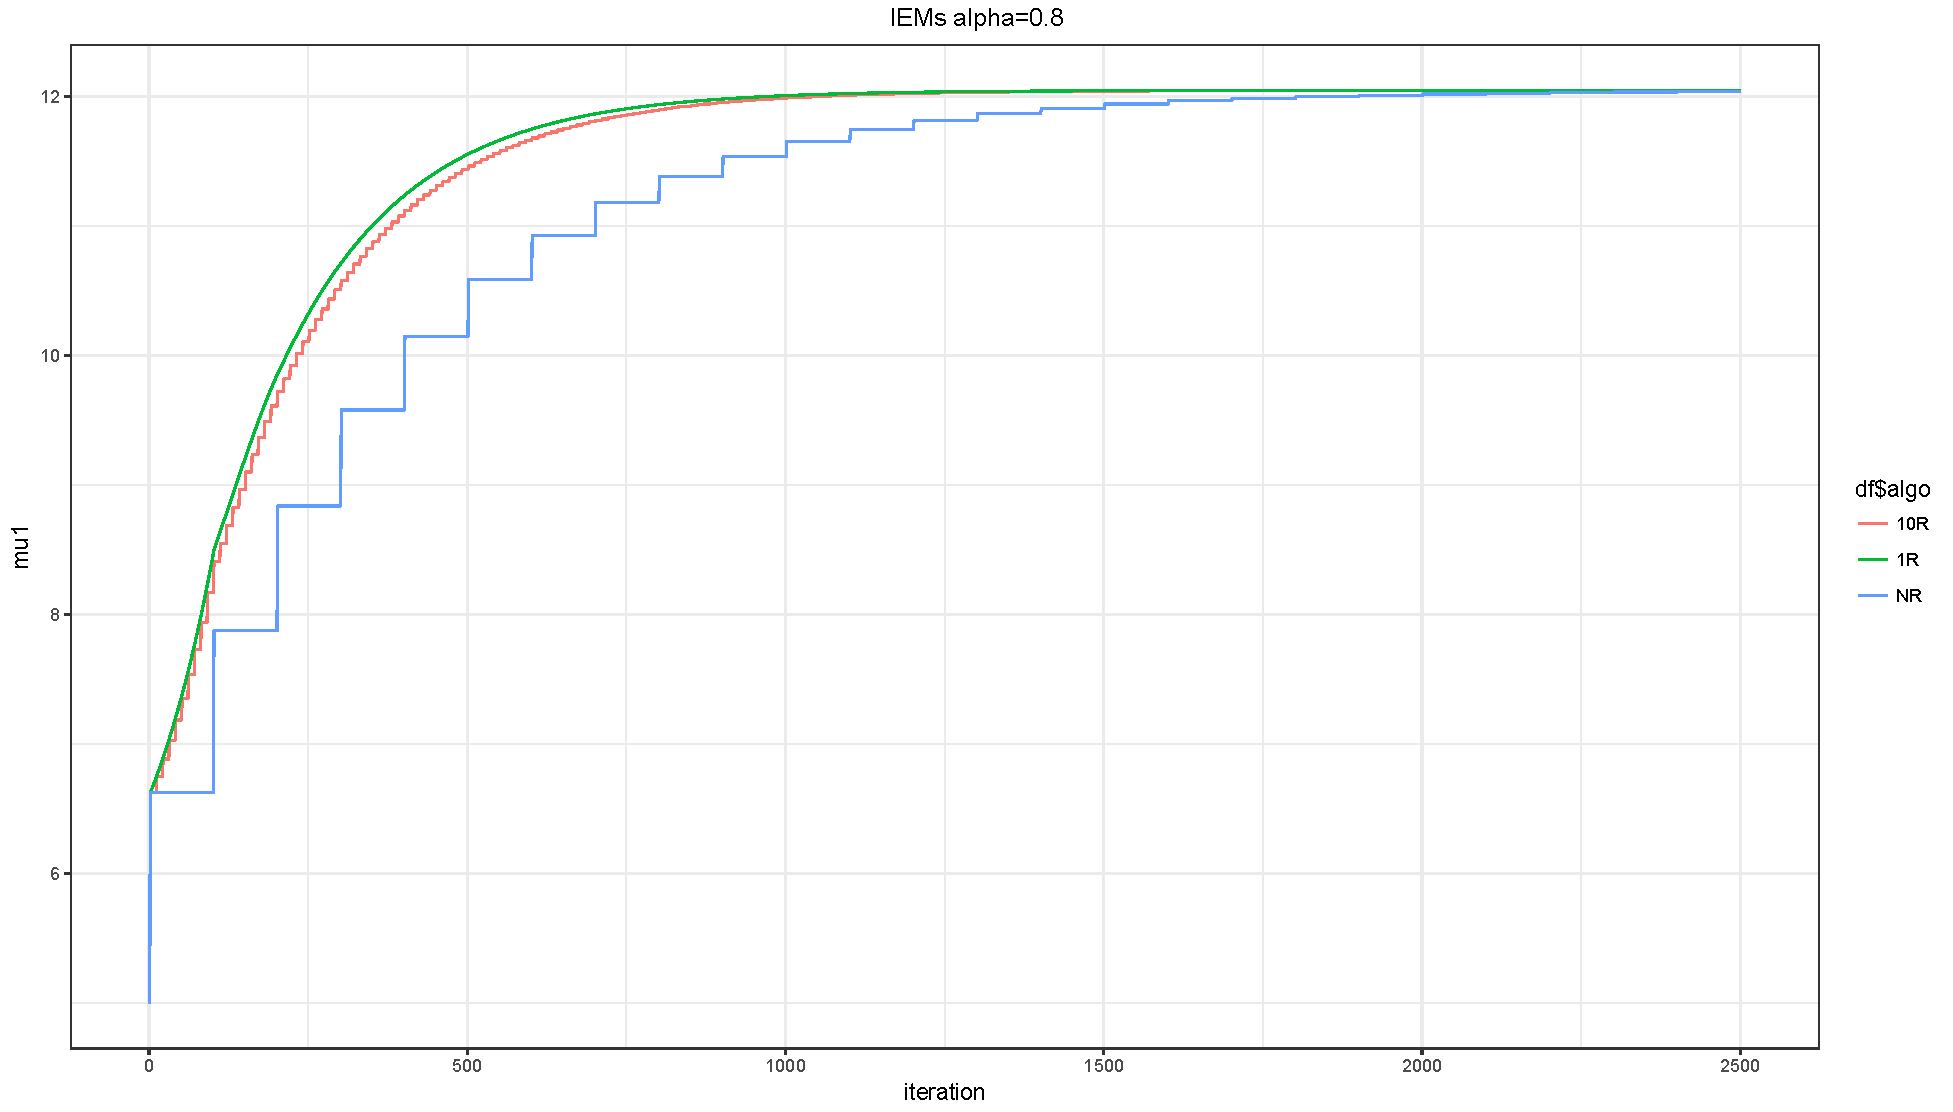
\includegraphics[scale=0.3]{iem_batch.pdf}
\end{center}
\end{figure}

We observe that the fastest convergence occurs when the batch size is minimal, i.E. $1$ individual per iteraiton.\\
This can be proven mathematically as well.\\
In the general case, where we consider that we pick pN individual at each iteration, where p is a percentage, then the general recurrent relation between parameter estimates is:
\begin{equation}
\theta_k = \rho^{1/p} \theta_{k-1/p} + (1-\alpha) \bar{y} e_1 \\
\end{equation}

What's really important here are the eigenvalues of $\rho$ at the power $\frac{1}{p}$. These are the values that will drive the speed of convergence. Even easier, the highest eigenvalue is enough to compare two algorithms (for two different values of p).\\
If we denote $g(p) = (\lambda_p)^{1/p}$ where $\lambda_p = max(eigenvalues(\rho_p))$ then the goal is to show the monotony of g(p).\\
Let's start by calculating the characteristic polynomial of $\rho$:
\begin{equation}
P_{\rho_p}(X) = (-1)^{1/p}(x^{1/p} - \alpha p \sum_{i=0}^{1/p-1}{X^i})
\end{equation}
Naturally $P_{\rho_p}(\lambda_p) = 0$ so:

\begin{equation}
\begin{split}
P_{\rho_p}(g(p)^p) & = 0\\
& = (-1)^{1/p}(g(p) - \alpha p \sum_{i=0}^{1/p-1}{(g(p)^{1/p})^i})
\end{split}
\end{equation}

Since $0 < g(p) < 1$ we have that :
\begin{equation}
\begin{split}
& (-1)^{1/p}(g(p) - \alpha p \sum_{i=0}^{1/p-1}{(g(p)^{1/p})^i}) = 0\\
& g(p) - \alpha p \frac{1 - g(p)}{1 - g(p)^p} = 0\\
& g(p)(1 - g(p)^p) = \alpha p (1 - g(p))
\end{split}
\end{equation}

We can derive this expression with respect to p and find:

\begin{equation}
\nabla g(p) \underbrace{(\overbrace{(1 - g(p)^p)}^{>0}- g(p)^p \overbrace{ln(g(p))}^{<0}p + \alpha p)}_{>0} = \underbrace{\alpha (1-g(p))}_{>0}
\end{equation}

Giving: 
\begin{equation}
\nabla g(p) > 0
\end{equation}

So g(p) is monotonic, so the speed of the IEM will be monotonic with the number of individual we pick at each iteration.


\subsection{MCEM and IMCEM}
In expectation ok all the same but bias variance tradeoff now.


\subsubsection{On the same simple case}
At iteration $N+j$, the vector of sufficient statistics remains the same as in the IEM.

\begin{equation}
S(y,z) = 
\left(
\begin{array}{c}
S(y_1,z_1) =z_1^{(N+j)}= z_1^{(N+1)}\\
..\\
S(y_j,z_j) =z_j^{(N+j)}= z_j^{(N+j)}\\
..\\
S(y_N,z_N) =z_N^{(N+j)}= z_N^{(N)}\\
\end{array}
\right)
\end{equation}

In the IMCEM, only the latent variable whose index has been picked will be simulated. Moreover, it will be simulated by the posterior distribution under the latest model parameter estimate. This distribution is the solution to the optimization problem induced by the Forward mapping. As a result we have:

\begin{equation}
z_j^{(N+j)} \sim p(z_j|y_j,\theta_{N+j-1})
\end{equation}
When i<j, each iteration N+i consisted in simulating the latent variable following:
\begin{equation}
z_i^{(N+i)} \sim p(z_i|y_i,\theta_{N+i-1})
\end{equation}
And when i>j, i.e. the individuals that are being picked afterwards (in the context of a sequential sampling of the individuals indices), the latent variables were simulated at the previous pass:
\begin{equation}
z_i^{(i)} \sim p(z_i|y_i,\theta_{i-1})
\end{equation}

In this case the posterior distribution being a Gaussian distribution we can write each latent variable as:
\begin{equation}
z_j = \alpha \theta{N+j-1} + (1-\alpha)y_j + e_{j,(N+j-1)}
\end{equation}
Where $e_{j,(N+j-1)} \sim \mathcal{N}(0, \gamma^2)$.\\

\noindent We can now apply our maximization step:
\begin{equation}
\begin{split}
& \theta_{(N+j)} = \hat{\Theta}(S) = \frac{\sum_{i=1}^{N}{\sum_{m=1}^{M_(N+j)}{(S(y_i,(z_i)^m)|y_i,\theta_{(N+j-i)})}}}{M_(N+j)N}\\
& = \frac{\alpha}{N} \sum_{i=1}^{N}{\theta_{N+j-i}} + (1-\alpha)\bar{y} + \bar{e}_{N+j}\\
\end{split}
\end{equation}
Where $\bar{e} \sim \mathcal{N}(0, \frac{\gamma^2}{M_(N+j)N})$

If we define the vector of parameter as follow (with $k=N+j$):

\begin{equation}
\theta_{k} = 
\left(
\begin{array}{c}
\theta_{k}\\
..\\
\theta_{k-N+1}\\
\end{array}
\right) = \rho \theta_{k-1} + (1-\alpha)\bar{y}e_1 + \bar{e}_k e_1
\end{equation}

Where:
\begin{equation}
\rho = \begin{pmatrix} 
\frac{\alpha}{N} & .. & .. & \frac{\alpha}{N} \\
1 & 0 & .. & 0\\
0 & 1 & .. & 0\\
.. & .. & .. & ..\\
.. & .. & .. & 0\\
\end{pmatrix}
\end{equation}
And:
\begin{equation}
e_1 = \begin{pmatrix} 
1\\
0\\
..\\
0\
\end{pmatrix} 
\end{equation}

\noindent Now if we consider a scheme where not only one individual is picked at each iteration but a batch pN (where p is a percentage). In that case we can write in scalar (to facilitate the notation we'll consider M=1 and $\bar{y} = 0$):
\begin{equation}
\begin{split}
\theta_k & = \rho^{1/p} \theta_{k-1/p} + \sum_{i=0}^{\rho^{i}}\bar{e}_k\\
& =  \rho^{1/p} \theta_{k-1/p} + \frac{1-\rho^{1/p}}{1-\rho}\bar{e}_k
\end{split}
\end{equation}
In that case we can calculate the expectation and the variance of our estimator $\theta_k$ in the stationary regime:
\begin{equation}
\begin{split}
& \E \theta_k = \rho^{k/p}\theta_0\\
& \textrm{Var } \theta_k = \frac{\gamma^2}{N(1-\rho)^2}\frac{1-\rho^{1/p}}{1+\rho^{1/p}}
\end{split}
\end{equation}

With these two expressions we understand what strategy is best for the choice of the batch size at each iteration. Indeed the bias is small when p is small so one should start with picking one individual first to kill the bias and the variance is decreasing when p is increasing. So once the bias is killed one should increase the size of the batch to kill the variance of the estimator.\\
\\
This result implies as well that the Online EM algorithm introduced by \citep{cappe} is the best strategy to follow even when all the data is initially available. In other words, even though one has access to the whole observed dataset, one should consider increasing batch of individuals at each iteration.

\begin{figure}[H]
\begin{center}
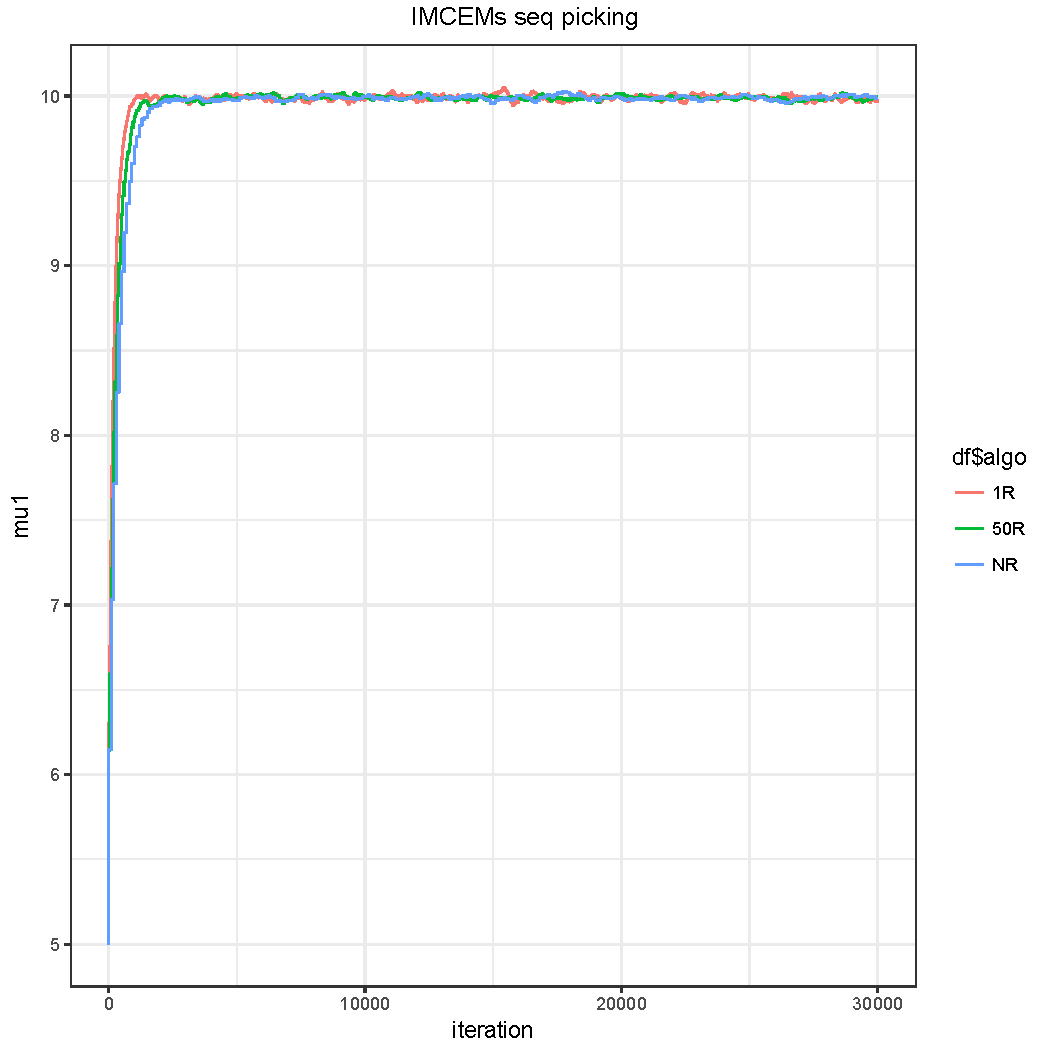
\includegraphics[scale=0.5]{imcem.pdf}
\end{center}
\end{figure}

Same results are shown for the ISAEM algorithm.

\subsubsection{2 components gaussian mixture}
Here the estimate model parameter at each iteration can be written as (after having written the posterior distirbution as a gradient)
\begin{equation}
\pi_k = \pi_{k-1} - P_k \frac{\partial \log p}{\partial \pi_k}
\end{equation}

Here we see that the monotony of the parameter, that was true in the previous case is no longer true here.
That's part of the reason why the sequential method is no longer the optimal and that the new algorithm presented priorly shows faster convergence. Nevertheless it seems that the uniform picking strategy is faster than the sequential one.

\begin{figure}[H]
\begin{center}
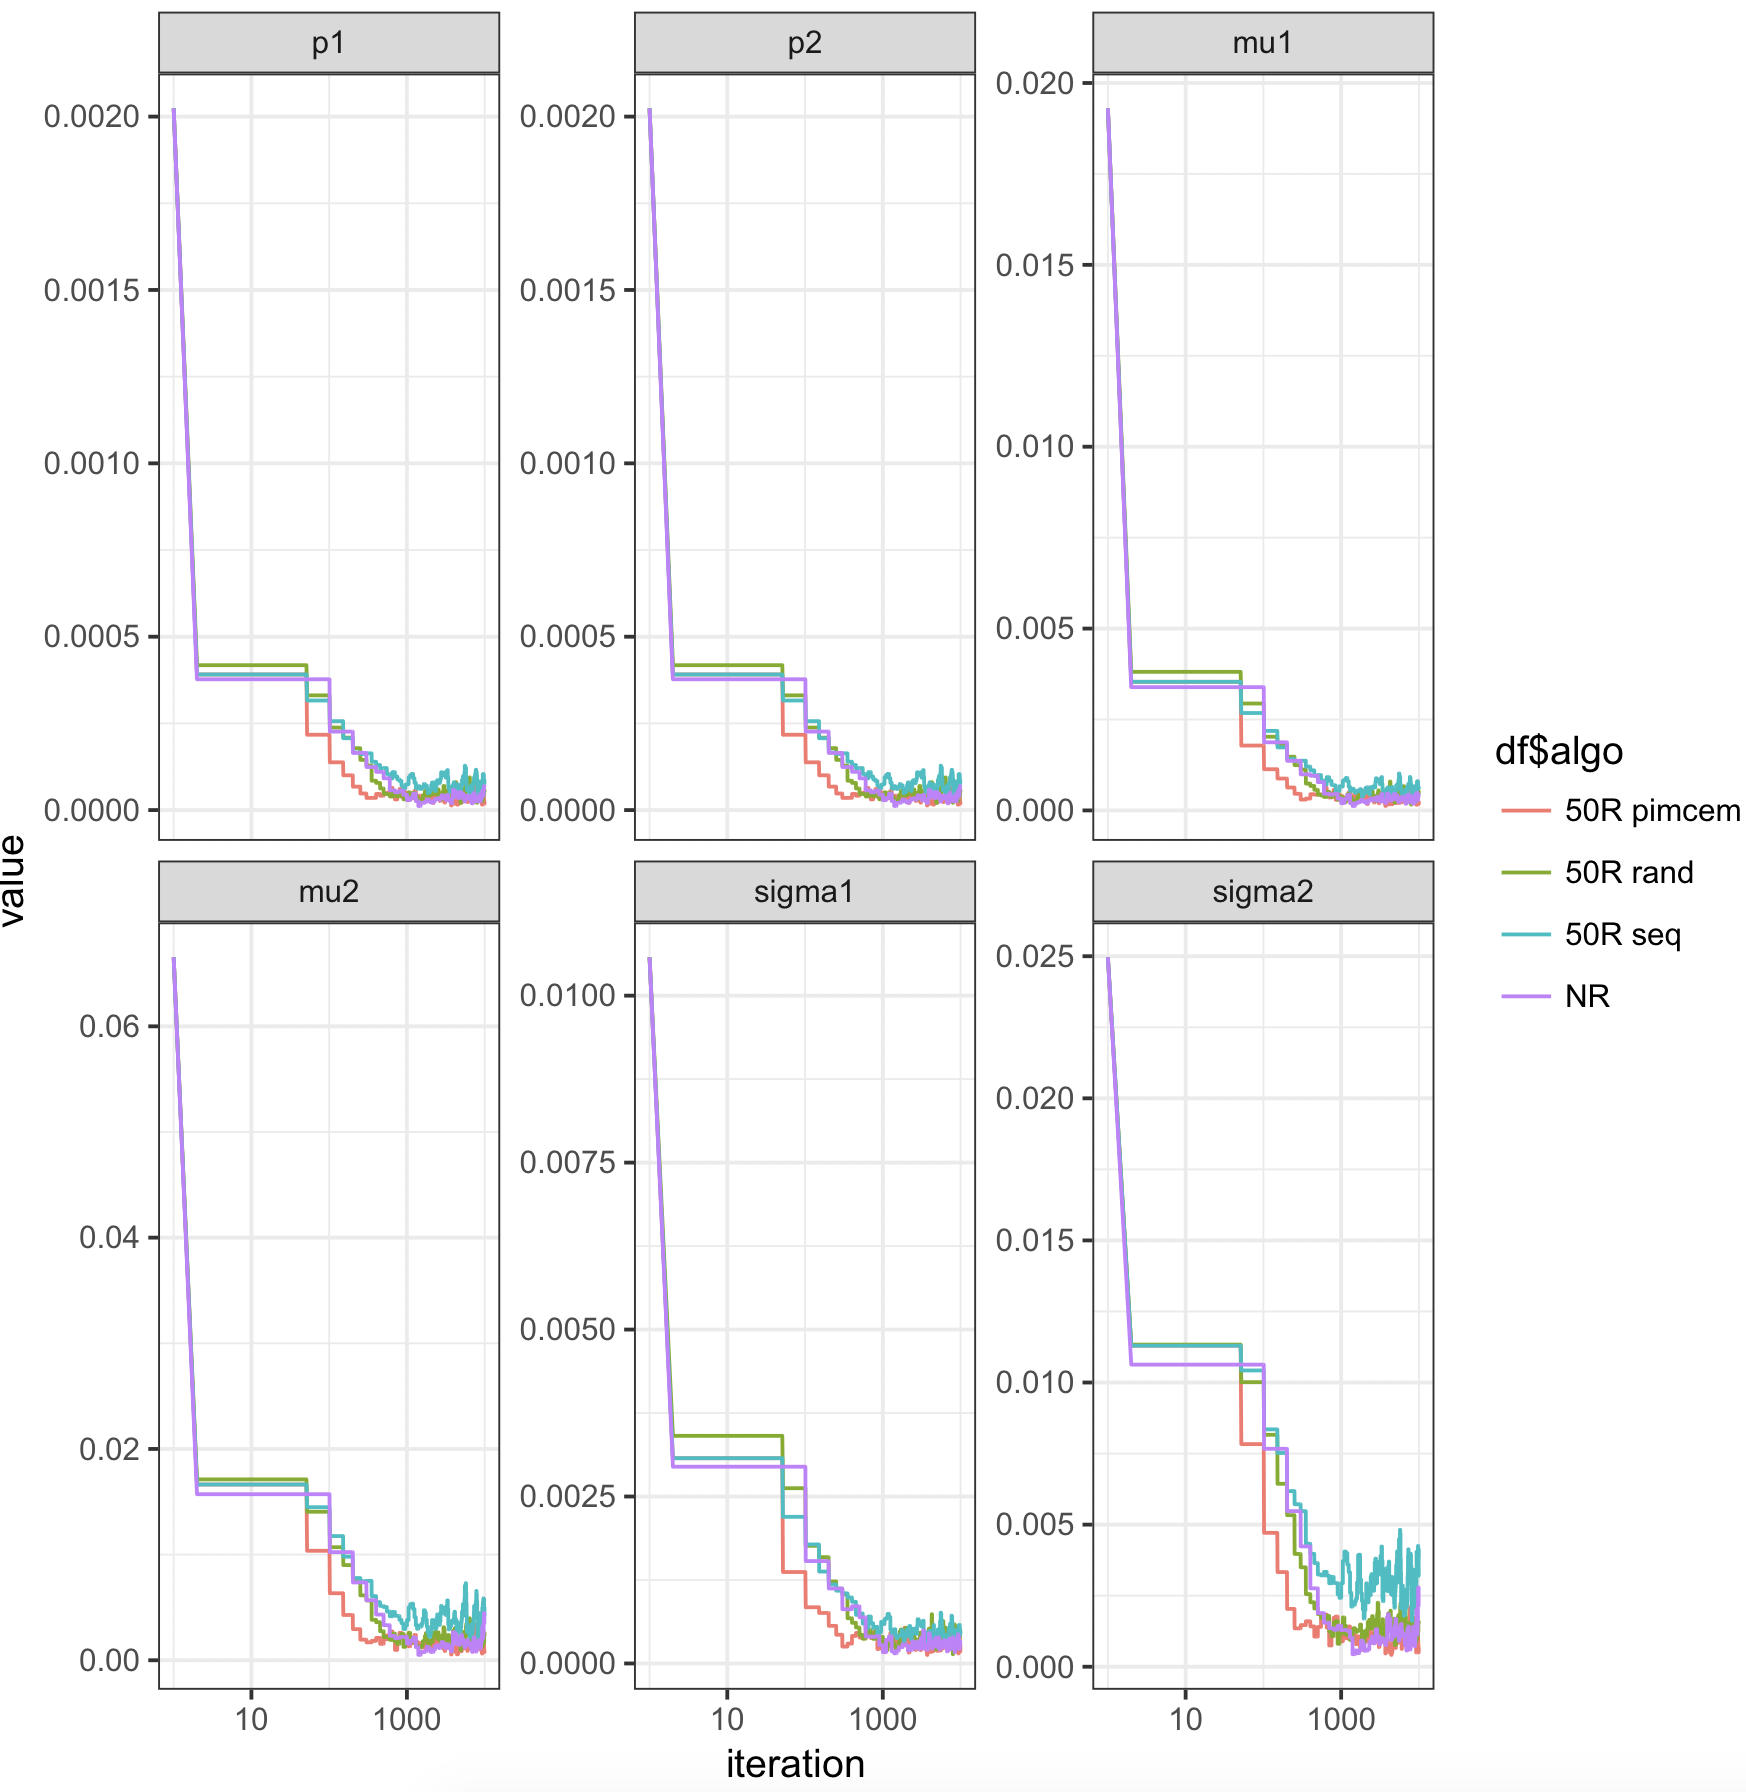
\includegraphics[scale=0.3]{imcem_2gmm.png}
\end{center}
\end{figure}
Also, the sequential method seems to show a bias.




\subsection{PK PD models}


%----------------------------------------------------------------------------------------
%   REFERENCE LIST
%----------------------------------------------------------------------------------------

\end{document}

